%%%%%%%%%%%%%%%%%%%%%%%%%%%%%%%%%%%%%%%%%
% Short Sectioned Assignment LaTeX Template Version 1.0 (5/5/12)
% This template has been downloaded from: http://www.LaTeXTemplates.com
% Original author:  Frits Wenneker (http://www.howtotex.com)
% License: CC BY-NC-SA 3.0 (http://creativecommons.org/licenses/by-nc-sa/3.0/)
%%%%%%%%%%%%%%%%%%%%%%%%%%%%%%%%%%%%%%%%%

%----------------------------------------------------------------------------------------
%	PACKAGES AND OTHER DOCUMENT CONFIGURATIONS
%----------------------------------------------------------------------------------------

\documentclass[paper=a4, fontsize=11pt]{scrartcl} % A4 paper and 11pt font size

% ---- Entrada y salida de texto -----


\usepackage[dvipsnames]{xcolor}
\usepackage{colortbl}
\usepackage{verbatim}
\usepackage{booktabs}
\usepackage{enumitem}
\newlist{subquestion}{enumerate}{1}
\setlist[subquestion,1]{label=(\alph*)}
\usepackage[T1]{fontenc} % Use 8-bit encoding that has 256 glyphs
\usepackage[utf8]{inputenc}
%\usepackage{fourier} % Use the Adobe Utopia font for the document - comment this line to return to the LaTeX default

% ---- Idioma --------

\usepackage[spanish, es-tabla]{babel} % Selecciona el español para palabras introducidas automáticamente, p.ej. "septiembre" en la fecha y especifica que se use la palabra Tabla en vez de Cuadro

% ---- Otros paquetes ----

\usepackage{url} % ,href} %para incluir URLs e hipervínculos dentro del texto (aunque hay que instalar href)
\usepackage{amsmath,amsfonts,amsthm} % Math packages
%\usepackage{graphics,graphicx, floatrow} %para incluir imágenes y notas en las imágenes
\usepackage{graphics,graphicx, float, subfig} %para incluir imágenes y colocarlas

% Para hacer tablas comlejas
%\usepackage{multirow}
%\usepackage{threeparttable}

%\usepackage{sectsty} % Allows customizing section commands
%\allsectionsfont{\centering \normalfont\scshape} % Make all sections centered, the default font and small caps

\usepackage{fancyhdr} % Custom headers and footers
\pagestyle{fancyplain} % Makes all pages in the document conform to the custom headers and footers
\usepackage{eurosym} % Para poder añadir el símbolo del euro
\fancyhead{} % No page header - if you want one, create it in the same way as the footers below
\fancyfoot[L]{} % Empty left footer
\fancyfoot[C]{} % Empty center footer
\fancyfoot[R]{\thepage} % Page numbering for right footer
\renewcommand{\headrulewidth}{0pt} % Remove header underlines
\renewcommand{\footrulewidth}{0pt} % Remove footer underlines
\setlength{\headheight}{13.6pt} % Customize the height of the header

\numberwithin{equation}{section} % Number equations within sections (i.e. 1.1, 1.2, 2.1, 2.2 instead of 1, 2, 3, 4)
\numberwithin{figure}{section} % Number figures within sections (i.e. 1.1, 1.2, 2.1, 2.2 instead of 1, 2, 3, 4)
\numberwithin{table}{section} % Number tables within sections (i.e. 1.1, 1.2, 2.1, 2.2 instead of 1, 2, 3, 4)

\setlength\parindent{0pt} % Removes all indentation from paragraphs - comment this line for an assignment with lots of text

\newcommand{\horrule}[1]{\rule{\linewidth}{#1}} % Create horizontal rule command with 1 argument of height


\usepackage{algpseudocode}
\usepackage[spanish]{babel}
\usepackage{varwidth}
\usepackage{hyperref}

\selectlanguage{spanish} 
\usepackage[spanish,onelanguage]{algorithm2e} %for psuedo code
\usepackage[lmargin=3.81cm,tmargin=2.54cm,rmargin=2.54cm,bmargin=2.52cm]{geometry}
%\usepackage{listings}
%\usepackage{dsfont}

%----------------------------------------------------------------------------------------
%	TÍTULO Y DATOS DEL ALUMNO
%----------------------------------------------------------------------------------------

\title{	
\normalfont \normalsize 
\textsc{\textbf{Metaheurísticas(2019-2020)} \\ Doble Grado en Ingeniería Informática y Matemáticas \\ Universidad de Granada} \\ [25pt] % Your university, school and/or department name(s)
\horrule{0.5pt} \\[0.4cm] % Thin top horizontal rule
\huge Técnicas de Búsqueda basadas en Poblaciones \\ para el Problema de la Máxima Diversidad  (MDP) \\ % The assignment title
\horrule{2pt} \\[0.5cm] % Thick bottom horizontal rule
}
\author{Alberto Jesús Durán López \\ 
DNI: 54142189-M \\
albduranlopez@gmail.com \\
\hfill \break \hspace{1cm}\\
Grupo Jueves, 17:30 - 19:30 } % Nombre y apellidos


\date{\normalsize\today} % Incluye la fecha actual

%----------------------------------------------------------------------------------------
% DOCUMENTO
%----------------------------------------------------------------------------------------

\begin{document}

\maketitle % Muestra el Título

\newpage %inserta un salto de página

\tableofcontents % para generar el índice de contenidos

% \listoffigures

% \listoftables

\newpage


\section{Introducción}
\hspace{1.5cm} Durante el transcurso de la asignatura se ha trabajado con el problema de la máxima diversidad \textit{(Max Diversity Problem)}. 


En particular, en esta práctica estudiaremos técnicas de búsqueda basadas en poblaciones para la resolución del problema en cuestión. \\
Comentaremos todos los pasos y problemas encontrados, detallando minuciosamente todos los detalles y soluciones a los mismos. \\

Además, se incorporarán tablas para mostrar los resultados de todas las ejecuciones y  gráficas para contrastar los modelos (optimización, costes y desviación).


\section{Problema de la máxima Diversidad}
\hspace{1.5cm} El problema de la máxima diversidad (\textit{maximum diversity problem}, MDP) es un problema de optimización combinatoria consistente en seleccionar un subconjunto de m elementos ($|M|=m$) de un conjunto inicial N de n elementos (con $n>m$) de forma que se maximice la diversidad entre los elementos escogidos. \\


El \textbf{MDP} se puede formular como: \\


\[
\text{Maximizar:   }  z_{MS}(x) = \sum_{i=1}^{n-1} \sum_{j=i+1}^{n} d_{ij}x_i x_j
\]



\[
\text{Sujeto a: } \sum_{i=1}^{n} x_i=m \hspace{0.2cm} \text{ con } x_i=\{0,1\} \text{, } i=1,...,n  \hspace{0.5cm} \text{donde: }
\]


\begin{itemize}
	\item x es una solución al problema que consiste en un vector binario que indica los m elementos seleccionados.
	\item $d_{ij}$ es la distancia existente entre los elementos $i$ y $j$
	
\end{itemize}


\begin{figure}[H]
	\centering
	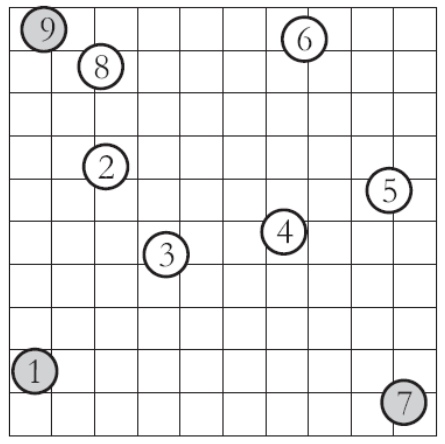
\includegraphics[scale=0.35]{img/mdp.png}
	\caption{MDP-Maximum Diversity Problem}
\end{figure}


\newpage
\section{Datos y casos considerados}
\hspace{1.5cm} Las ejecuciones se han realizado en un ordenador \texttt{Intel(R) Core(TM) i7-1065G7 CPU @ 1.30GHz, 16GB RAM, 512 SSD}. 


Se utilizarán \textbf{30 casos} seleccionados de varios de los conjuntos de instancias disponible en la \href{http://www.optsicom.es/mdp/}{MDPLIB}, 10 pertenecientes al grupo \texttt{GKD} con distancias Euclideas, n=500 y m=50 \textit{(GKD-c\_11\_n500\_m50 a GKD-
c\_20\_n500\_m50)}, 10 del grupo \texttt{MDG} con distancias reales en [0,1000], n=500 y m=50
\textit{(MDG-b\_1\_n500\_m50 a MDG-b\_10\_n500\_m50)}; y otras 10 del grupo \texttt{MDG} con distancias enteras en {0,10}, n=2000 y m=200 \textit{(MDG-a\_31\_n2000\_m200 a MDG-
a\_40\_n2000\_m200)}. \\


Para la realización de la práctica usaremos el lenguaje de programación \texttt{C++} ya que se deben probar muchos ejemplos y la ejecución es más rápida al ser un lenguaje de programación compilado. \\
Todos los archivos se han compilado con la opción de optimización \texttt{-O2} y, además,  la semilla usada para todas
las ejecuciones ha sido 54142189, pudiéndose ésta indicar en la ejecución del archivo en cuestión. 





\subsection{Esquema de representación de soluciones}

Para todos los algoritmos menos para la \textit{Búsqueda Local}, se ha usado una codificación basada en números binarios. Sin embargo, dejaremos la explicación para las siguientes secciones, donde se explicará con detalle en cada algoritmo.


\subsection{Descripción de la Función Objetivo}

Todos los algoritmos implementados hacen uso de la misma función objetivo, la comentada en el punto (2) anterior y cuyo pseudocódigo mostramos a continuación. Bien es cierto que en el caso de la \textit{Búsqueda Local} se tiene que usar codificación basada en números enteros, sin embargo, dicha función se ve mínimamente modificada.


\begin{figure}[H]
	\centering
	\begin{minipage}{.9\linewidth}
		
		
		
		\begin{algorithm}[H] 
			

			\SetAlgoLined
			
			\KwData{\textbf{ContribucionIndep}(\textit{integer ind, vector sel, matriz distancias)}}
			
			\Begin{
				\textit{suma $\leftarrow$ 0} \;
				
				\For{j in sel}{
					$ suma \leftarrow sel[j]\cdot(distancias[ind][j] + suma)$ \;	
				}
				
				\Return $suma$
			}
			
		\end{algorithm} 
		
	\end{minipage}
\end{figure}



\begin{figure}[H]
	\centering
	\begin{minipage}{.9\linewidth}
		
		
		
		\begin{algorithm}[H] 
			
			\caption{Evaluar solución}
			\SetAlgoLined
			
			\KwData{\textbf{CosteEstimado}(\textit{vector sel, matriz distancias)}}
			
			\Begin{
				
				\textit{suma $\leftarrow$ 0} \;
				
				
				\For{i in $|sel|$}{
					\If{$sel[i]=true$}{
						$ suma \leftarrow ContribucionIndep(i, sel, distancias) + suma$ \;
					}
					
				}
				
				\Return $suma/2$
			}
			
		\end{algorithm} 
		
	\end{minipage}
\end{figure}









\section{Enfriamiento Simulado}

\hspace{1.5cm}Para el desarrollo del \textit{Enfriamiento Simulado}, dividimos su explicación en distintas componentes:

\begin{itemize}
	\item \texttt{Esquema de representación y solución inicial}: Para este algoritmo se ha usado una codificación basada en números binarios, 1 si se toma el elemento y 0 	en caso contrario. Almacenamos la solución en un conjunto \textit{sel} y,  nuestro algoritmo que genera las soluciones iniciales, se encargará de crear dichos valores comprobando que se cumplan las restricciones (el número de unos debe ser igual a \texttt{m}).
	
	\item \texttt{Parámetros y esquema de enfriamiento}: 
	La temperatura inicial ($T_0$) y final ($T_f$) se calculan de la siguiente forma:
	
	\[  
		T_0 = \frac{\mu \cdot C(s_0)}{-ln(\phi)}   \text{    ;} \hspace{1cm} T_f = 10^{-3}
	\]
	
	donde $\phi \in [0,1]$ es la probabilidad de aceptar una solución un $\mu$ por 1 peor que la inicial, cumpliendo  $\mu = \phi = 0.3$ para nuestro caso. 
	
	
	$C(S_0)$ es el coste de la solución inicial 
	
	
	Por otro lado, para el enfriamiento se ha empleado el esquema de Cauchy Modificado, donde $\beta$ es una constante que calcularemos al principio de nuestro algoritmo y $T_{k+1}$ se calculará en cada iteración.
	
	\[  
	T_{k+1} = \frac{T_k}{1 + \beta \cdot T_k} \hspace{0.35cm} \text{con} \hspace{0.35cm} \beta = \frac{T_0 - T_f}{M \cdot T_0\cdot T_f}   
	\]
	donde M es el número de enfriamientos a realizar.
	
	\item \texttt{Esquema de generación de vecinos}:
	El entorno de una solución \textit{sel} está formado por las soluciones accesibles desde ella a través de un movimiento de intercambio.
	En cada iteración, se aplicará un movimiento de intercambio \textbf{Int}\textit{(sel,i,j)} que consistirá en intercambiar un elemento i por j en el contenedor de seleccionados(se cambiarán elementos diferentes, 1 por 0). El gran número de intercambios supone un gran número de llamadas a la función objetivo y, en consecuencia, una peor eficiencia. Por ello, realizamos una factorización de la función objetivo, de forma que sólo tengamos que sumar y restar las contribuciones del elemento añadido y quitado, respectivamente.
\end{itemize}



\newpage

Mostramos a continuación el pseudocódigo asociado a la función principal de nuestro algoritmo:
\begin{figure}[H]
	\centering
	\begin{minipage}{.95\linewidth}
		
		
		
		\begin{algorithm}[H] 
			
			\caption{Enfriamiento Simulado}
			\SetAlgoLined
			
			\KwData{\textbf{ES}(\textit{integer m, matriz distancias)}}
			
			\Begin{
				
				
				$max\_vecinos \leftarrow 10 \cdot n$ \;
				$max\_exitos \leftarrow 0.1 \cdot max\_vecinos$ \;
				$evaluaciones \leftarrow 100000$ \;
				$enfriamientos \leftarrow 100000 \cdot max\_vecinos$ \;
				
				
				\hfill
				
				\textit{sel $\leftarrow$} \textbf{Solucion Aleatoria}(\textit{n,m}) \;
				$t_0 \leftarrow (\mu \cdot Coste(sel))/-ln(\phi)$ \;
				$t_f \leftarrow 1/1000$ \;
				
				$\beta \leftarrow (t_0-t_f)/(enfriamientos \cdot t_0 \cdot t_f) $ \;
				
				
				\hfill
				
				\While{$t_f<t_0$ and $eval<evaluaciones$ and $exitos \not = 0$ }{
					\textit{exitos $\leftarrow$ 0} \;
					
					\For{$i=0$; $i<max\_vecinos$ and $exitos<max\_exitos$; $i++$}{
						\textit{siguiente $\leftarrow$ Intercambio(sel, i, j)} \;
						$eval++$ \;
						
						\textit{$dif$ $\leftarrow$ Contribución Nueva - Contribución Vieja} \;
						\break \hfill
						
						
						\If{$dif >0$ or $U(0,1) < exp(dif/t_0$)}{
							$exitos++$ \;
							\textit{Coste(Siguiente) $\leftarrow$ Coste(Siguiente) + $dif$} \;
							\textit{sel $\leftarrow$ siguiente} \;
							
							\hfill
							
							\If{$Coste(Siguiente) > Coste(mejor\_sol)$}{
								\textit{mejor\_sol $\leftarrow$ siguiente} \;
							}
						}
					}
					$t_0 \leftarrow t_0/(1+ \beta \cdot t_0) $\;
				}
				
			}
			
		\end{algorithm} 
		
	\end{minipage}
\end{figure}

\newpage

\section{Búsqueda Local}
\hspace{1.5cm}El algoritmo de \textit{Búsqueda Local} usado para el resto de algoritmos que se explican en las siguientes secciones se corresponde con el implementado en la primera práctica, por ello, conviene recordar como funciona: 

\begin{itemize}
	
	

\item En nuestro problema MDP, el parámetro \texttt{i} indica el índice del elemento que se eliminará de la solución y el j por cual se sustituirá. Por tanto, las opciones para \texttt{i} serán \texttt{m} (los m elementos seleccionados) y las opciones para \texttt{j} serán \texttt{n-m} (los elementos disponibles en \textit{no seleccionados}), por tanto, el entorno estará formado por \texttt{m$\cdot$(n-m)} elementos.


	
	\begin{figure}[H]
		\centering
		\begin{minipage}{.75\linewidth}
			
			\begin{algorithm}[H] 
				\caption{EvaluaVecinos }
				\SetAlgoLined
				
				\KwData{\textbf{EvaluaVecinos}}
				
				
				\Begin{
					
					$mejora \leftarrow True$\;
					$eval \leftarrow 0$ \;
					
					\break \hfill
					
					
					\While{\textit{eval<100.000 and mejora}}{
						
						
						
						\break \hfill
						
						\hspace{3cm}\textbf{. . .}
						
						
						
						\break \hfill
						
						$salir \leftarrow$ False, $c \leftarrow 0$ \;
						
						\While{$c< n-m$ and not salir}{
							
							\textit{Genera elemento válido j} \;
							
							\If{\texttt{Contrib($s_j$)}>\texttt{Contrib($s_i$)}}{
								
								\textit{Int(sel, i, j)} \;
								$salir \leftarrow$ True\;
								$coste\leftarrow coste + contribNueva - contribAntigua$ 
							}
							$c\leftarrow c+1$\;
							$eval\leftarrow eval+1$\;
						}
					}
				}
			\end{algorithm}
		\end{minipage}
	\end{figure}
	
	
\item En cada iteración, podemos calcular la diferencia de costes entre las dos soluciones recalculando todas las distancias de la función objetivo, sin embargo, esto no es necesario ya que como únicamente añadimos y quitamos 1 elemento, basta con sumar y restar la distancia del nuevo y del viejo elemento al resto de elementos seleccionados, respectivamente. Además, combinamos la factorización del coste con el cálculo de la contribución de los elementos para mejorar aún más la eficiencia.



Si el intercambio es favorable, es decir, si el coste de la nueva solución (sumando las distancias del nuevo elemento y restando las del elemento anterior) es mayor que la anterior, aceptamos el intercambio. En caso contrario, rechazamos.

\item Repetiremos este proceso hasta que se realicen \textit{N} evaluaciones de la función objetivo o cuando no encuentre mejora en el entorno.

\end{itemize}








\newpage 
\section{Búsqueda Multiarranque Básica}
\hspace{1.5cm}El algoritmo de \textit{BMB} es quizás el algoritmo menos laborioso de nuestra práctica. Éste, consistirá en generar 10 soluciones iniciales aleatorias que serán optimizadas con nuestra \textit{Búsqueda Local} implementada en la práctica 1 y descrita en el apartado anterior.

\texttt{Criterio de parada}: el algoritmo finalizará cuando no encuentre mejora en todo el entorno o cuando se hayan realizado 10.000 evaluaciones de la función objetivo. \\


Mostramos la función asociada a la generación de soluciones iniciales. Como en nuestro algoritmo simplemente tenemos que aplicar la \textit{Búsqueda Local}, usamos codificación basada en conjuntos enteros.
\begin{figure}[H]
	\centering
	\begin{minipage}{.8\linewidth}
		
		\begin{algorithm}[H] 
			
			\caption{Solución inicial}
			\SetAlgoLined
			
			\KwData{\textbf{Solucion Inicial}$(n,m)$}
			
			\Begin{
				\textit{vector<int>}  \textit{sel} \;
				
				\While{\textit{$sel \not = m$}}{
					
					$random \leftarrow rand()\%n$ \;
					
					\If{random no insertado}{
						$sel \leftarrow sel \cup random$ \;
					}
				}
				
				\Return $sel$
			}
			
		\end{algorithm} 
		
	\end{minipage}
\end{figure}





Por último, mostramos el pseudocódigo asociado a la función principal. Se realiza un bucle \textbf{for} para realizar un total de 10 iteraciones en las que se generarán soluciones aleatorias y se le aplicará \textit{BL}. La solución devuelta será la mejor de todas.


\begin{figure}[H]
	\centering
	\begin{minipage}{.8\linewidth}
		
		\begin{algorithm}[H] 
			
			\caption{Búsqueda Multiarranque Básica}
			\SetAlgoLined
			
			\KwData{\textbf{BMB}(\textit{integer m, matriz distancias)}}
			
			\Begin{
				
				\textit{total $\leftarrow$ 10} \;
				\textit{matriz soluciones(total)} \;
				\textit{vector mejor} \;
				\hfill \break 
				\For{i=0 to $total$}{
					\textit{soluciones[i]} $\leftarrow$ \textbf{Solución Aleatoria(n,m)} \;
					\textit{soluciones[i] $\leftarrow$ \textbf{BusquedaLocal}(\textit{soluciones[i], distancias}}) \;
					
					
					\If{$Coste(soluciones[i])>Coste(mejor)$}{
						$ mejor \leftarrow soluciones[i]$ \;
					}
					
				}
			}
			
		\end{algorithm} 
		
	\end{minipage}
\end{figure}



\newpage
\section{Búsqueda Local Reiterada (ILS)}

\hspace{1.5cm}Este algoritmo combina Búsqueda \textit{Local} con mutación. En cata iteración se aplicará \textit{BL} y mutación sobre la mejor solución encontrada y, tras un número de iteraciones, se devolverá la mejor solución encontrada en toda la ejecución. Es decir, se sigue el criterio del mejor como aceptación de la \textit{ILS}.

\subsection{Generación de Soluciones Iniciales}
El esquema de la solución inicial, al igual que la práctica anterior, está caracterizado por la codificación binaria. Cada solución estará formada por valores booleanos 1 (cuando se toma el elemento) o 0 (en caso contrario). 

Mostramos a continuación el algoritmo para la generación aleatoria de la solución inicial, teniendo en cuenta que debe cumplir las restricciones del problema MDP, es decir, que el número de 1 es igual a \texttt{m}.

\begin{figure}[H]
	\centering
	\begin{minipage}{.8\linewidth}
		
		
		
		\begin{algorithm}[H] 
			
			\caption{Solución inicial}
			\SetAlgoLined
			
			\KwData{\textbf{Solucion Inicial}$(n,m)$}
			
			\Begin{
				\textit{vector<bool>}  \textit{sel(n)} \;
				
				
				\While{$total \not = m$}{
					$i\leftarrow rand()\%n$ \;
					$sel[i] \leftarrow true$ \;
					
					$total \leftarrow $ \textit{nº de True en sel} \;
				}
				
				\Return $sel$
			}
			
		\end{algorithm} 
		
	\end{minipage}
\end{figure}










\subsection{Esquema de Búsqueda ILS, ILS-ES}



El operador de mutación de \textit{ILS} se basa en un operador de vecino para representación de orden que provoca un cambio brusco en la solución actual. Dicho cambio, será mayor que el considerado en la \textit{BL}, realizándose un total de $m \cdot 0.1$ mutaciones. 


\begin{figure}[H]
	\centering
	\begin{minipage}{.8\linewidth}
		
		
		
		\begin{algorithm}[H] 
			
			\caption{Operador de Mutación}
			\SetAlgoLined
			
			\KwData{\textbf{Operador Mutación}$(sel,m)$}
			
			\Begin{
				$total \leftarrow m\cdot$\textit{0.1} \;
				
				
				\While{$total>0$}{
					$i \leftarrow $ \textit{Generar índice} \;
					
					\textbf{hacer}\{ \hfill \break
						\text{    }$j \leftarrow $ \textit{Generar índice} \;
					\}\textbf{mientras}($sel[i]=sel[j]$) \;
					
					
					\textit{Intercambiar sel[i] por sel[j]}\;
					\textit{total - -} \;
				}
				
				\Return $sel$
			}
			
		\end{algorithm} 
		
	\end{minipage}
\end{figure}

\newpage

En total, se han implementado 2 versiones, ambas caracterizadas por realizar 10 iteraciones donde se aplicará 10 veces el algoritmo de \textit{BL} (la primera sobre una solución inicial aleatoria y las 9 restantes sobre mutaciones mutadas).

\begin{itemize}
	\item \texttt{ILS}: Para el algoritmo de \textit{Búsqueda Local} se ha usado el implementado en la práctica 1 y descrito anteriormente.
	
	
	
	\item \texttt{ILS-ES}: Tiene la misma composición que el \textit{ILS} estándar, con la única diferencia que el algoritmo de \textit{Búsqueda Local} considerado es el \textit{ES} implementado en la primera parte de la práctica.
\end{itemize}

EL pseudocódigo para ambas versiones es el siguiente:

\begin{figure}[H]
	\centering
	\begin{minipage}{.8\linewidth}
		
		\begin{algorithm}[H] 
			
			\caption{Búsqueda Local Reiterada}
			\SetAlgoLined
			
			\KwData{\textbf{ILS}(\textit{integer m, matriz distancias)}}
			
			\Begin{
				
				\textit{totalBL $\leftarrow$ 10} \;
				\textit{inicial} $\leftarrow$ \textbf{Solucion Inicial}(\textit{n,m}) \;
				
				\textit{sel} $\leftarrow$ \textbf{Busqueda Local}(\textit{inicial}) \;
				\textit{totalBL - -} \;
				
				
				\hfill \break 
				\While{$totalBL>0$}{
					
					
					\textit{sel} $\leftarrow$ \textbf{OperadorMutacion}(\textit{sel,m})\;
					
					\textit{sel} $\leftarrow$ \textbf{Busqueda Local}(\textit{sel, distancias}) \;

					\textit{totalBL - -} \;
					
					
					\If{$Coste(sel)>Coste(mejor)$}{
						$ mejor \leftarrow sel$ \;
					}\Else{
						$ sel \leftarrow mejor$ \;
					}
					
				}
			}
			
		\end{algorithm} 
		
	\end{minipage}
\end{figure}



\section{Resultados Obtenidos}













% Please add the following required packages to your document preamble:
% \usepackage{booktabs}
% \usepackage{graphicx}
% \usepackage[table,xcdraw]{xcolor}
% If you use beamer only pass "xcolor=table" option, i.e. \documentclass[xcolor=table]{beamer}
\begin{table}[H]
	\centering
	\resizebox{\textwidth}{!}{%
		\begin{tabular}{@{}
				>{\columncolor[HTML]{FFFFFF}}c 
				>{\columncolor[HTML]{FFFFFF}}c 
				>{\columncolor[HTML]{FFFFFF}}c 
				>{\columncolor[HTML]{FFFFFF}}c 
				>{\columncolor[HTML]{FFFFFF}}c 
				>{\columncolor[HTML]{FFFFFF}}c 
				>{\columncolor[HTML]{FFFFFF}}c 
				>{\columncolor[HTML]{FFFFFF}}c @{}}
			\toprule
			{\color[HTML]{333333} \textbf{Instancia}}     & {\color[HTML]{333333} \textbf{Mejor Coste}} & {\color[HTML]{333333} \textbf{ES}} & {\color[HTML]{333333} \textbf{Desv}} & {\color[HTML]{333333} \textbf{Time}} & {\color[HTML]{333333} \textbf{BMB}} & {\color[HTML]{333333} \textbf{Desv}} & {\color[HTML]{333333} \textbf{Time}} \\ \midrule
			{\color[HTML]{333333} GKD-c\_11\_n500\_m50}   & {\color[HTML]{333333} 19587,13}             & {\color[HTML]{333333} 19581,2}     & {\color[HTML]{333333} 0,03}          & {\color[HTML]{333333} 0,03}          & {\color[HTML]{333333} 19586}        & {\color[HTML]{333333} 0,01}          & {\color[HTML]{333333} 0,03}          \\
			{\color[HTML]{333333} GKD-c\_12\_n500\_m50}   & {\color[HTML]{333333} 19360,24}             & {\color[HTML]{333333} 19357}       & {\color[HTML]{333333} 0,02}          & {\color[HTML]{333333} 0,04}          & {\color[HTML]{333333} 19360,2}      & {\color[HTML]{333333} 0,00}          & {\color[HTML]{333333} 0,05}          \\
			{\color[HTML]{333333} GKD-c\_13\_n500\_m50}   & {\color[HTML]{333333} 19366,70}             & {\color[HTML]{333333} 19366,7}     & {\color[HTML]{333333} 0,00}          & {\color[HTML]{333333} 0,03}          & {\color[HTML]{333333} 19366,7}      & {\color[HTML]{333333} 0,00}          & {\color[HTML]{333333} 0,04}          \\
			{\color[HTML]{333333} GKD-c\_14\_n500\_m50}   & {\color[HTML]{333333} 19458,56}             & {\color[HTML]{333333} 19453,1}     & {\color[HTML]{333333} 0,03}          & {\color[HTML]{333333} 0,04}          & {\color[HTML]{333333} 19458,6}      & {\color[HTML]{333333} 0,00}          & {\color[HTML]{333333} 0,04}          \\
			{\color[HTML]{333333} GKD-c\_15\_n500\_m50}   & {\color[HTML]{333333} 19422,15}             & {\color[HTML]{333333} 19418,6}     & {\color[HTML]{333333} 0,02}          & {\color[HTML]{333333} 0,03}          & {\color[HTML]{333333} 19421,6}      & {\color[HTML]{333333} 0,00}          & {\color[HTML]{333333} 0,03}          \\
			{\color[HTML]{333333} GKD-c\_16\_n500\_m50}   & {\color[HTML]{333333} 19680,21}             & {\color[HTML]{333333} 19665,2}     & {\color[HTML]{333333} 0,08}          & {\color[HTML]{333333} 0,02}          & {\color[HTML]{333333} 19680,2}      & {\color[HTML]{333333} 0,00}          & {\color[HTML]{333333} 0,04}          \\
			{\color[HTML]{333333} GKD-c\_17\_n500\_m50}   & {\color[HTML]{333333} 19331,39}             & {\color[HTML]{333333} 19327,3}     & {\color[HTML]{333333} 0,02}          & {\color[HTML]{333333} 0,03}          & {\color[HTML]{333333} 19331,4}      & {\color[HTML]{333333} 0,00}          & {\color[HTML]{333333} 0,03}          \\
			{\color[HTML]{333333} GKD-c\_18\_n500\_m50}   & {\color[HTML]{333333} 19461,39}             & {\color[HTML]{333333} 19459,8}     & {\color[HTML]{333333} 0,01}          & {\color[HTML]{333333} 0,03}          & {\color[HTML]{333333} 19461,4}      & {\color[HTML]{333333} 0,00}          & {\color[HTML]{333333} 0,03}          \\
			{\color[HTML]{333333} GKD-c\_19\_n500\_m50}   & {\color[HTML]{333333} 19477,39}             & {\color[HTML]{333333} 19471,6}     & {\color[HTML]{333333} 0,03}          & {\color[HTML]{333333} 0,04}          & {\color[HTML]{333333} 19477,3}      & {\color[HTML]{333333} 0,00}          & {\color[HTML]{333333} 0,04}          \\
			{\color[HTML]{333333} GKD-c\_20\_n500\_m50}   & {\color[HTML]{333333} 19604,84}             & {\color[HTML]{333333} 19601,8}     & {\color[HTML]{333333} 0,02}          & {\color[HTML]{333333} 0,05}          & {\color[HTML]{333333} 19604,8}      & {\color[HTML]{333333} 0,00}          & {\color[HTML]{333333} 0,04}          \\
			{\color[HTML]{333333} MDG-b\_1\_n500\_m50}    & {\color[HTML]{333333} 778030,62}            & {\color[HTML]{333333} 762432}      & {\color[HTML]{333333} 2,00}          & {\color[HTML]{333333} 0,07}          & {\color[HTML]{333333} 768472}       & {\color[HTML]{333333} 1,23}          & {\color[HTML]{333333} 0,04}          \\
			{\color[HTML]{333333} MDG-b\_2\_n500\_m50}    & {\color[HTML]{333333} 779963,69}            & {\color[HTML]{333333} 764288}      & {\color[HTML]{333333} 2,01}          & {\color[HTML]{333333} 0,05}          & {\color[HTML]{333333} 771856}       & {\color[HTML]{333333} 1,04}          & {\color[HTML]{333333} 0,04}          \\
			{\color[HTML]{333333} MDG-b\_3\_n500\_m50}    & {\color[HTML]{333333} 776768,44}            & {\color[HTML]{333333} 763946}      & {\color[HTML]{333333} 1,65}          & {\color[HTML]{333333} 0,05}          & {\color[HTML]{333333} 767181}       & {\color[HTML]{333333} 1,23}          & {\color[HTML]{333333} 0,04}          \\
			{\color[HTML]{333333} MDG-b\_4\_n500\_m50}    & {\color[HTML]{333333} 775394,62}            & {\color[HTML]{333333} 766680}      & {\color[HTML]{333333} 1,12}          & {\color[HTML]{333333} 0,06}          & {\color[HTML]{333333} 765863}       & {\color[HTML]{333333} 1,23}          & {\color[HTML]{333333} 0,04}          \\
			{\color[HTML]{333333} MDG-b\_5\_n500\_m50}    & {\color[HTML]{333333} 775611,06}            & {\color[HTML]{333333} 753849}      & {\color[HTML]{333333} 2,81}          & {\color[HTML]{333333} 0,02}          & {\color[HTML]{333333} 770415}       & {\color[HTML]{333333} 0,67}          & {\color[HTML]{333333} 0,04}          \\
			{\color[HTML]{333333} MDG-b\_6\_n500\_m50}    & {\color[HTML]{333333} 775153,69}            & {\color[HTML]{333333} 759891}      & {\color[HTML]{333333} 1,97}          & {\color[HTML]{333333} 0,05}          & {\color[HTML]{333333} 765810}       & {\color[HTML]{333333} 1,21}          & {\color[HTML]{333333} 0,04}          \\
			{\color[HTML]{333333} MDG-b\_7\_n500\_m50}    & {\color[HTML]{333333} 777232,87}            & {\color[HTML]{333333} 762001}      & {\color[HTML]{333333} 1,96}          & {\color[HTML]{333333} 0,04}          & {\color[HTML]{333333} 766665}       & {\color[HTML]{333333} 1,36}          & {\color[HTML]{333333} 0,04}          \\
			{\color[HTML]{333333} MDG-b\_8\_n500\_m50}    & {\color[HTML]{333333} 779168,75}            & {\color[HTML]{333333} 764350}      & {\color[HTML]{333333} 1,90}          & {\color[HTML]{333333} 0,05}          & {\color[HTML]{333333} 773351}       & {\color[HTML]{333333} 0,75}          & {\color[HTML]{333333} 0,04}          \\
			{\color[HTML]{333333} MDG-b\_9\_n500\_m50}    & {\color[HTML]{333333} 774802,19}            & {\color[HTML]{333333} 756551}      & {\color[HTML]{333333} 2,36}          & {\color[HTML]{333333} 0,03}          & {\color[HTML]{333333} 766528}       & {\color[HTML]{333333} 1,07}          & {\color[HTML]{333333} 0,03}          \\
			{\color[HTML]{333333} MDG-b\_10\_n500\_m50}   & {\color[HTML]{333333} 774961,31}            & {\color[HTML]{333333} 759213}      & {\color[HTML]{333333} 2,03}          & {\color[HTML]{333333} 0,05}          & {\color[HTML]{333333} 771090}       & {\color[HTML]{333333} 0,50}          & {\color[HTML]{333333} 0,04}          \\
			{\color[HTML]{333333} MDG-a\_31\_n2000\_m200} & {\color[HTML]{333333} 114139}               & {\color[HTML]{333333} 112544}      & {\color[HTML]{333333} 1,40}          & {\color[HTML]{333333} 0,41}          & {\color[HTML]{333333} 113028}       & {\color[HTML]{333333} 0,97}          & {\color[HTML]{333333} 0,67}          \\
			{\color[HTML]{333333} MDG-a\_32\_n2000\_m200} & {\color[HTML]{333333} 114092}               & {\color[HTML]{333333} 112382}      & {\color[HTML]{333333} 1,50}          & {\color[HTML]{333333} 0,50}          & {\color[HTML]{333333} 112651}       & {\color[HTML]{333333} 1,26}          & {\color[HTML]{333333} 0,65}          \\
			{\color[HTML]{333333} MDG-a\_33\_n2000\_m200} & {\color[HTML]{333333} 114124}               & {\color[HTML]{333333} 112426}      & {\color[HTML]{333333} 1,49}          & {\color[HTML]{333333} 0,49}          & {\color[HTML]{333333} 112944}       & {\color[HTML]{333333} 1,03}          & {\color[HTML]{333333} 0,65}          \\
			{\color[HTML]{333333} MDG-a\_34\_n2000\_m200} & {\color[HTML]{333333} 114203}               & {\color[HTML]{333333} 112573}      & {\color[HTML]{333333} 1,43}          & {\color[HTML]{333333} 0,43}          & {\color[HTML]{333333} 112835}       & {\color[HTML]{333333} 1,20}          & {\color[HTML]{333333} 0,63}          \\
			{\color[HTML]{333333} MDG-a\_35\_n2000\_m200} & {\color[HTML]{333333} 114180}               & {\color[HTML]{333333} 112820}      & {\color[HTML]{333333} 1,19}          & {\color[HTML]{333333} 0,44}          & {\color[HTML]{333333} 112944}       & {\color[HTML]{333333} 1,08}          & {\color[HTML]{333333} 0,64}          \\
			{\color[HTML]{333333} MDG-a\_36\_n2000\_m200} & {\color[HTML]{333333} 114252}               & {\color[HTML]{333333} 112386}      & {\color[HTML]{333333} 1,63}          & {\color[HTML]{333333} 0,47}          & {\color[HTML]{333333} 112987}       & {\color[HTML]{333333} 1,11}          & {\color[HTML]{333333} 0,64}          \\
			{\color[HTML]{333333} MDG-a\_37\_n2000\_m200} & {\color[HTML]{333333} 114213}               & {\color[HTML]{333333} 112244}      & {\color[HTML]{333333} 1,72}          & {\color[HTML]{333333} 0,43}          & {\color[HTML]{333333} 112874}       & {\color[HTML]{333333} 1,17}          & {\color[HTML]{333333} 0,65}          \\
			{\color[HTML]{333333} MDG-a\_38\_n2000\_m200} & {\color[HTML]{333333} 114378}               & {\color[HTML]{333333} 112921}      & {\color[HTML]{333333} 1,27}          & {\color[HTML]{333333} 0,40}          & {\color[HTML]{333333} 112991}       & {\color[HTML]{333333} 1,21}          & {\color[HTML]{333333} 0,65}          \\
			{\color[HTML]{333333} MDG-a\_39\_n2000\_m200} & {\color[HTML]{333333} 114201}               & {\color[HTML]{333333} 112209}      & {\color[HTML]{333333} 1,74}          & {\color[HTML]{333333} 0,41}          & {\color[HTML]{333333} 112908}       & {\color[HTML]{333333} 1,13}          & {\color[HTML]{333333} 0,64}          \\
			{\color[HTML]{333333} MDG-a\_40\_n2000\_m200} & {\color[HTML]{333333} 114191}               & {\color[HTML]{333333} 112819}      & {\color[HTML]{333333} 1,20}          & {\color[HTML]{333333} 0,40}          & {\color[HTML]{333333} 112834}       & {\color[HTML]{333333} 1,19}          & {\color[HTML]{333333} 0,65}          \\ \bottomrule
		\end{tabular}%
	}
	\caption{Resultados ES/BMB}
	\label{AMallo2}
\end{table}








% Please add the following required packages to your document preamble:
% \usepackage{booktabs}
% \usepackage{graphicx}
% \usepackage[table,xcdraw]{xcolor}
% If you use beamer only pass "xcolor=table" option, i.e. \documentclass[xcolor=table]{beamer}
\begin{table}[H]
	\centering
	\resizebox{\textwidth}{!}{%
		\begin{tabular}{@{}
				>{\columncolor[HTML]{FFFFFF}}c 
				>{\columncolor[HTML]{FFFFFF}}c 
				>{\columncolor[HTML]{FFFFFF}}c 
				>{\columncolor[HTML]{FFFFFF}}c 
				>{\columncolor[HTML]{FFFFFF}}c 
				>{\columncolor[HTML]{FFFFFF}}c 
				>{\columncolor[HTML]{FFFFFF}}c 
				>{\columncolor[HTML]{FFFFFF}}c @{}}
			\toprule
			{\color[HTML]{333333} \textbf{Instancia}}     & {\color[HTML]{333333} \textbf{Mejor Coste}} & {\color[HTML]{330001} \textbf{ILS}} & {\color[HTML]{330001} \textbf{Desv}} & {\color[HTML]{330001} \textbf{Time}} & {\color[HTML]{330001} \textbf{ILS-ES}} & {\color[HTML]{330001} \textbf{Desv}} & {\color[HTML]{330001} \textbf{Time}} \\ \midrule
			{\color[HTML]{330001} GKD-c\_11\_n500\_m50}   & {\color[HTML]{330001} 19587,13}             & {\color[HTML]{333333} 19587,1}      & {\color[HTML]{333333} 0,00}          & {\color[HTML]{333333} 0,03}          & {\color[HTML]{333333} 19584,6}         & {\color[HTML]{333333} 0,01}          & {\color[HTML]{333333} 0,31}          \\
			{\color[HTML]{330001} GKD-c\_12\_n500\_m50}   & {\color[HTML]{330001} 19360,24}             & {\color[HTML]{333333} 19360,2}      & {\color[HTML]{333333} 0,00}          & {\color[HTML]{333333} 0,04}          & {\color[HTML]{333333} 19360,2}         & {\color[HTML]{333333} 0,00}          & {\color[HTML]{333333} 0,32}          \\
			{\color[HTML]{330001} GKD-c\_13\_n500\_m50}   & {\color[HTML]{330001} 19366,70}             & {\color[HTML]{333333} 19366,7}      & {\color[HTML]{333333} 0,00}          & {\color[HTML]{333333} 0,05}          & {\color[HTML]{333333} 19366,7}         & {\color[HTML]{333333} 0,00}          & {\color[HTML]{333333} 0,32}          \\
			{\color[HTML]{330001} GKD-c\_14\_n500\_m50}   & {\color[HTML]{330001} 19458,56}             & {\color[HTML]{333333} 19458,6}      & {\color[HTML]{333333} 0,00}          & {\color[HTML]{333333} 0,03}          & {\color[HTML]{333333} 19458,6}         & {\color[HTML]{333333} 0,00}          & {\color[HTML]{333333} 0,29}          \\
			{\color[HTML]{330001} GKD-c\_15\_n500\_m50}   & {\color[HTML]{330001} 19422,15}             & {\color[HTML]{333333} 19421,6}      & {\color[HTML]{333333} 0,00}          & {\color[HTML]{333333} 0,03}          & {\color[HTML]{333333} 19422,1}         & {\color[HTML]{333333} 0,00}          & {\color[HTML]{333333} 0,33}          \\
			{\color[HTML]{330001} GKD-c\_16\_n500\_m50}   & {\color[HTML]{330001} 19680,21}             & {\color[HTML]{333333} 19680,2}      & {\color[HTML]{333333} 0,00}          & {\color[HTML]{333333} 0,03}          & {\color[HTML]{333333} 19680,2}         & {\color[HTML]{333333} 0,00}          & {\color[HTML]{333333} 0,32}          \\
			{\color[HTML]{330001} GKD-c\_17\_n500\_m50}   & {\color[HTML]{330001} 19331,39}             & {\color[HTML]{333333} 19331,4}      & {\color[HTML]{333333} 0,00}          & {\color[HTML]{333333} 0,04}          & {\color[HTML]{333333} 19329,4}         & {\color[HTML]{333333} 0,01}          & {\color[HTML]{333333} 0,29}          \\
			{\color[HTML]{330001} GKD-c\_18\_n500\_m50}   & {\color[HTML]{330001} 19461,39}             & {\color[HTML]{333333} 19461,4}      & {\color[HTML]{333333} 0,00}          & {\color[HTML]{333333} 0,04}          & {\color[HTML]{333333} 19461,4}         & {\color[HTML]{333333} 0,00}          & {\color[HTML]{333333} 0,35}          \\
			{\color[HTML]{330001} GKD-c\_19\_n500\_m50}   & {\color[HTML]{330001} 19477,39}             & {\color[HTML]{333333} 19477,3}      & {\color[HTML]{333333} 0,00}          & {\color[HTML]{333333} 0,03}          & {\color[HTML]{333333} 19477,3}         & {\color[HTML]{333333} 0,00}          & {\color[HTML]{333333} 0,32}          \\
			{\color[HTML]{330001} GKD-c\_20\_n500\_m50}   & {\color[HTML]{330001} 19604,84}             & {\color[HTML]{333333} 19604,8}      & {\color[HTML]{333333} 0,00}          & {\color[HTML]{333333} 0,04}          & {\color[HTML]{333333} 19604,8}         & {\color[HTML]{333333} 0,00}          & {\color[HTML]{333333} 0,34}          \\
			{\color[HTML]{330001} MDG-b\_1\_n500\_m50}    & {\color[HTML]{330001} 778030,62}            & {\color[HTML]{333333} 768893}       & {\color[HTML]{333333} 1,17}          & {\color[HTML]{333333} 0,04}          & {\color[HTML]{333333} 770455}          & {\color[HTML]{333333} 0,97}          & {\color[HTML]{333333} 0,59}          \\
			{\color[HTML]{330001} MDG-b\_2\_n500\_m50}    & {\color[HTML]{330001} 779963,69}            & {\color[HTML]{333333} 776145}       & {\color[HTML]{333333} 0,49}          & {\color[HTML]{333333} 0,04}          & {\color[HTML]{333333} 768793}          & {\color[HTML]{333333} 1,43}          & {\color[HTML]{333333} 0,38}          \\
			{\color[HTML]{330001} MDG-b\_3\_n500\_m50}    & {\color[HTML]{330001} 776768,44}            & {\color[HTML]{333333} 769205}       & {\color[HTML]{333333} 0,97}          & {\color[HTML]{333333} 0,05}          & {\color[HTML]{333333} 768283}          & {\color[HTML]{333333} 1,09}          & {\color[HTML]{333333} 0,65}          \\
			{\color[HTML]{330001} MDG-b\_4\_n500\_m50}    & {\color[HTML]{330001} 775394,62}            & {\color[HTML]{333333} 769641}       & {\color[HTML]{333333} 0,74}          & {\color[HTML]{333333} 0,04}          & {\color[HTML]{333333} 767491}          & {\color[HTML]{333333} 1,02}          & {\color[HTML]{333333} 0,45}          \\
			{\color[HTML]{330001} MDG-b\_5\_n500\_m50}    & {\color[HTML]{330001} 775611,06}            & {\color[HTML]{333333} 769000}       & {\color[HTML]{333333} 0,85}          & {\color[HTML]{333333} 0,03}          & {\color[HTML]{333333} 765396}          & {\color[HTML]{333333} 1,32}          & {\color[HTML]{333333} 0,38}          \\
			{\color[HTML]{330001} MDG-b\_6\_n500\_m50}    & {\color[HTML]{330001} 775153,69}            & {\color[HTML]{333333} 759684}       & {\color[HTML]{333333} 2,00}          & {\color[HTML]{333333} 0,04}          & {\color[HTML]{333333} 768544}          & {\color[HTML]{333333} 0,85}          & {\color[HTML]{333333} 0,47}          \\
			{\color[HTML]{330001} MDG-b\_7\_n500\_m50}    & {\color[HTML]{330001} 777232,87}            & {\color[HTML]{333333} 765951}       & {\color[HTML]{333333} 1,45}          & {\color[HTML]{333333} 0,06}          & {\color[HTML]{333333} 769574}          & {\color[HTML]{333333} 0,99}          & {\color[HTML]{333333} 0,50}          \\
			{\color[HTML]{330001} MDG-b\_8\_n500\_m50}    & {\color[HTML]{330001} 779168,75}            & {\color[HTML]{333333} 775018}       & {\color[HTML]{333333} 0,53}          & {\color[HTML]{333333} 0,04}          & {\color[HTML]{333333} 771452}          & {\color[HTML]{333333} 0,99}          & {\color[HTML]{333333} 0,54}          \\
			{\color[HTML]{330001} MDG-b\_9\_n500\_m50}    & {\color[HTML]{330001} 774802,19}            & {\color[HTML]{333333} 770633}       & {\color[HTML]{333333} 0,54}          & {\color[HTML]{333333} 0,05}          & {\color[HTML]{333333} 769227}          & {\color[HTML]{333333} 0,72}          & {\color[HTML]{333333} 0,50}          \\
			{\color[HTML]{330001} MDG-b\_10\_n500\_m50}   & {\color[HTML]{330001} 774961,31}            & {\color[HTML]{333333} 766173}       & {\color[HTML]{333333} 1,13}          & {\color[HTML]{333333} 0,05}          & {\color[HTML]{333333} 769320}          & {\color[HTML]{333333} 0,73}          & {\color[HTML]{333333} 0,45}          \\
			{\color[HTML]{330001} MDG-a\_31\_n2000\_m200} & {\color[HTML]{330001} 114139}               & {\color[HTML]{333333} 113825}       & {\color[HTML]{333333} 0,28}          & {\color[HTML]{333333} 0,41}          & {\color[HTML]{333333} 113008}          & {\color[HTML]{333333} 0,99}          & {\color[HTML]{333333} 4,21}          \\
			{\color[HTML]{330001} MDG-a\_32\_n2000\_m200} & {\color[HTML]{330001} 114092}               & {\color[HTML]{333333} 113268}       & {\color[HTML]{333333} 0,72}          & {\color[HTML]{333333} 0,46}          & {\color[HTML]{333333} 112858}          & {\color[HTML]{333333} 1,08}          & {\color[HTML]{333333} 4,23}          \\
			{\color[HTML]{330001} MDG-a\_33\_n2000\_m200} & {\color[HTML]{330001} 114124}               & {\color[HTML]{333333} 113223}       & {\color[HTML]{333333} 0,79}          & {\color[HTML]{333333} 0,43}          & {\color[HTML]{333333} 113062}          & {\color[HTML]{333333} 0,93}          & {\color[HTML]{333333} 4,70}          \\
			{\color[HTML]{330001} MDG-a\_34\_n2000\_m200} & {\color[HTML]{330001} 114203}               & {\color[HTML]{333333} 113306}       & {\color[HTML]{333333} 0,79}          & {\color[HTML]{333333} 0,38}          & {\color[HTML]{333333} 112887}          & {\color[HTML]{333333} 1,15}          & {\color[HTML]{333333} 4,55}          \\
			{\color[HTML]{330001} MDG-a\_35\_n2000\_m200} & {\color[HTML]{330001} 114180}               & {\color[HTML]{333333} 113838}       & {\color[HTML]{333333} 0,30}          & {\color[HTML]{333333} 0,37}          & {\color[HTML]{333333} 112966}          & {\color[HTML]{333333} 1,06}          & {\color[HTML]{333333} 4,87}          \\
			{\color[HTML]{330001} MDG-a\_36\_n2000\_m200} & {\color[HTML]{330001} 114252}               & {\color[HTML]{333333} 113220}       & {\color[HTML]{333333} 0,90}          & {\color[HTML]{333333} 0,39}          & {\color[HTML]{333333} 113002}          & {\color[HTML]{333333} 1,09}          & {\color[HTML]{333333} 4,81}          \\
			{\color[HTML]{330001} MDG-a\_37\_n2000\_m200} & {\color[HTML]{330001} 114213}               & {\color[HTML]{333333} 113447}       & {\color[HTML]{333333} 0,67}          & {\color[HTML]{333333} 0,38}          & {\color[HTML]{333333} 112946}          & {\color[HTML]{333333} 1,11}          & {\color[HTML]{333333} 4,39}          \\
			{\color[HTML]{330001} MDG-a\_38\_n2000\_m200} & {\color[HTML]{330001} 114378}               & {\color[HTML]{333333} 113427}       & {\color[HTML]{333333} 0,83}          & {\color[HTML]{333333} 0,37}          & {\color[HTML]{333333} 113016}          & {\color[HTML]{333333} 1,19}          & {\color[HTML]{333333} 4,62}          \\
			{\color[HTML]{330001} MDG-a\_39\_n2000\_m200} & {\color[HTML]{330001} 114201}               & {\color[HTML]{333333} 113589}       & {\color[HTML]{333333} 0,54}          & {\color[HTML]{333333} 0,38}          & {\color[HTML]{333333} 112761}          & {\color[HTML]{333333} 1,26}          & {\color[HTML]{333333} 4,34}          \\
			{\color[HTML]{330001} MDG-a\_40\_n2000\_m200} & {\color[HTML]{330001} 114191}               & {\color[HTML]{333333} 113398}       & {\color[HTML]{333333} 0,69}          & {\color[HTML]{333333} 0,39}          & {\color[HTML]{333333} 112959}          & {\color[HTML]{333333} 1,08}          & {\color[HTML]{333333} 4,61}          \\ \bottomrule
		\end{tabular}%
	}
	\caption{Resultados ILS}
	\label{AMallo}
\end{table}




\[
\begin{array}{r|*{4}{r}}{Algoritmo}&Desv&Tiempo\\\hline


{}Greedy&1,36&0,46\\

{}BL&1,07&0.49\\

{}ES&1,15&0,17\\

{}BMB&0,72&0,24\\

{}ILS&0,55&0,16\\

{}ILS\text{-}ES&0,70&1,78
\end{array}
\label{glob}
\]


\newpage
\section{Análisis de Resultados}

\begin{itemize}

\item Observando la tabla de resultados globales \ref{glob} anterior, el algoritmo \textit{Greedy} es con el que peor resultados se obtienen. El resto de algoritmos considerados tienen una desviación que se encuentra en un rango de valores muy óptimo y ajustado.

\item Por otro lado, todos los algoritmos son muy eficientes, con un tiempo de ejecución de media por debajo de 1 segundo, a excepción de \textit{ILS-ES} que casi dobla este valor.


\item Dejando el \textit{Greedy} de lado, obtenemos dos grupos de algoritmos, los que están basados en trayectorias simples (\textit{BL y ES}) y los que están basados en trayectorias múltiples (\textit{BMB, ILS e ILS-ES}), caracterizados por ejecutar las técnicas de trayectorias simples varias veces.

Teniendo en cuenta este punto, los resultados obtenidos cuadran con el razonamiento teórico, ya que \textit{BMB, ILS e ILS-ES} reducen en torno al 40\% la desviación obtenida de las técnicas basadas en trayectorias simples. 
\end{itemize}








Recordemos los casos seleccionados para la ejecución de los algoritmos:
Mostramos los resultados obtenidos en gráficas diferentes según el grupo al que pertenezca cada instancia para reflejar mejor las diferencias:



\begin{itemize}
	\item \texttt{GKD-c}: Conjunto de datos, referentes al grupo de distancias Euclideas con $n=500$, $m=50$,  en el que mejor resultados se han obtenido, tanto los algoritmos basados en técnicas de trayectorias simples como múltiples llegan al mejor coste.  Hay convergencia con todos algoritmos en todas las instancias, de hecho, se aprecia que todas las líneas están superpuestas, obteniendo prácticamente una desviación nula.
	
	
	\begin{figure}[H]
		\centering
		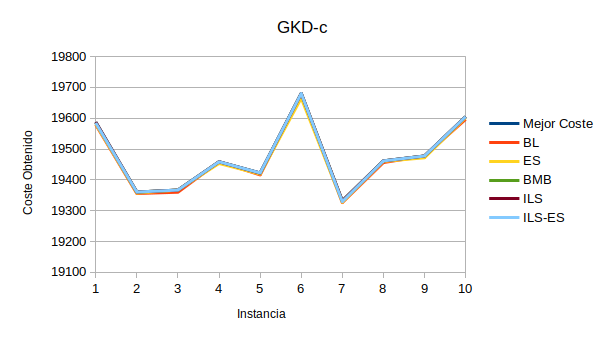
\includegraphics[scale=0.62]{img/gkdc.png}
	\end{figure}
	
	
	\newpage 
	
	\item \texttt{MDG-a}: Conjunto de datos correspondiente al grupo de distancias enteras y tamaño de $n=2000$ y $m=200$. En todas las instancias los costes obtenidos por los algoritmos basados en técnicas de trayectorias múltiples superan a los que están basados en técnicas de trayectorias simples. 
	Se aprecia como la línea de \textit{ILS} se encuentra por encima del resto, mientras la roja y amarilla, pertenecientes a los algoritmos \textit{BL y ES}, se encuentran por debajo.
	
	

	
	
	\begin{figure}[H]
		\centering
		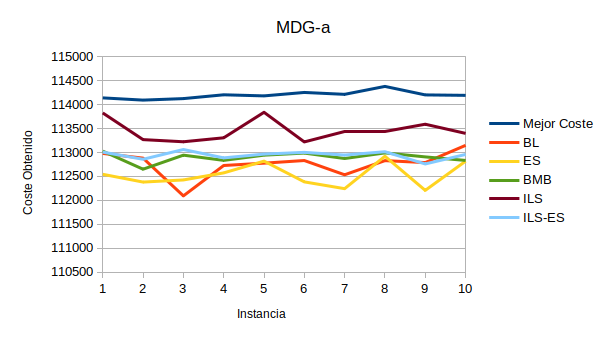
\includegraphics[scale=0.62]{img/mdga.png}
	\end{figure}
	
	
	
	\item \texttt{MDG-b}: Conjunto de datos correspondiente al grupo de distancias reales y tamaño $n=500$ y $m=50$. 
	Al igual que en el grupo de instancias anterior, los algoritmos basados en trayectorias simples (\textit{BL} y \textit{ES}) se encuentran por debajo del resto.
	
	Si observamos el trazado por cada uno de los algoritmos, observamos que se presentan altibajos o fluctuaciones en las mismas instancias. Esto es debido a la presencia de óptimos locales, haciendo costoso que nuestros algoritmos puedan salir de estos. 
	
	

	\begin{figure}[H]
		\centering
		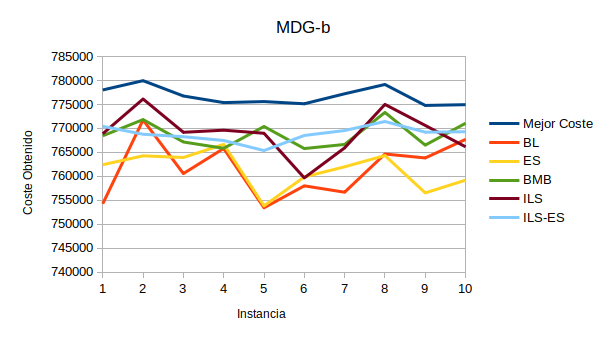
\includegraphics[scale=0.62]{img/mdgb.png}
	\end{figure}
	
\end{itemize}

\newpage

Un aspecto diferente en los algoritmos implementados radica en el número de soluciones usadas en el proceso de optimización. \textit{Enfriamiento Simulado} o \textit{Búsqueda Local} utilizan una sola solución en el proceso de búsqueda. \\



Por otro lado, técnicas como \textit{Búsqueda Multiarranque Básica} o \textit{Búsqueda Local Reiterada} optimizan un conjunto de soluciones iniciales creadas de forma aleatoria por lo que se obtienen soluciones de más calidad debido a la ventaja que supone explorar diferentes áreas del espacio de búsqueda.

Debido a la posible presencia de óptimos locales, algoritmos como \textit{Búsqueda Local Reiterada} (\textit{ILS}) presentan un factor de mutación brusco, mejorando en gran medida los resultados obtenidos.







\subsection{Desviación}
Por último, reflejados en el siguiente gráfico en red, mostramos la desviación obtenida de todas las instancia tras la ejecución de cada algoritmo. Como bien sabemos, cuanto menor sea la desviación, mejor será el coste obtenido con nuestro algoritmo. Por tanto, el algoritmo que presente un mayor área bajo su trazado, será peor.




\begin{figure}[H]
	\centering
	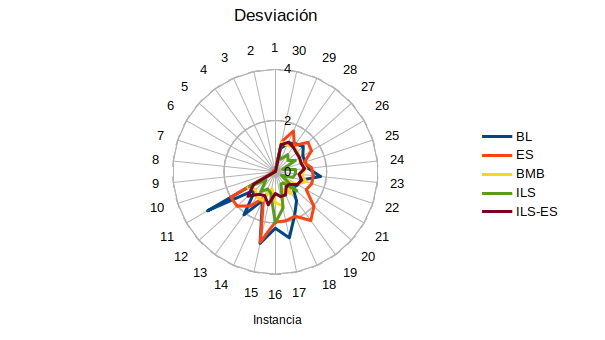
\includegraphics[scale=0.6]{img/desv.png}
	
\end{figure}



En resumen, podemos considerar que tanto la eficacia como la eficiencia de todos nuestros algoritmos es muy buena por tener una desviación y un tiempo muy pequeños.

Con los que mejor resultados se obtienen son con los algoritmos basados en técnicas de trayectorias múltiples, especialmente el algoritmo de \textit{Búsqueda Local Reiterada} (\textit{ILS}) ya que en media obtiene soluciones más cercanas al mejor valor conocido.









\newpage
\begin{thebibliography}{X} 
	
-\href{https://sci2s.ugr.es/sites/default/files/files/Teaching/GraduatesCourses/Metaheuristicas/Sem01-Problemas-MHs-2019-20.pdf}{Seminario 1}\\
	
	-\href{https://sci2s.ugr.es/sites/default/files/files/Teaching/GraduatesCourses/Metaheuristicas/Sem02-Problemas-BusquedaLocal-MHs-19-20.pdf}{Seminario 2}\\
	
		-\href{https://sci2s.ugr.es/sites/default/files/Sem03-Problemas-Poblaciones-MHs-19-20.pdf}{Seminario 3}\\
		
		-\href{https://sci2s.ugr.es/sites/default/files/files/Teaching/GraduatesCourses/Metaheuristicas/Sem04-Problemas-Trayectorias-MHs-19-20.pdf}{Seminario 4}\\
	
	-\href{https://sci2s.ugr.es/sites/default/files/files/Teaching/GraduatesCourses/Metaheuristicas/Guion\%20P3a\%20Trayectorias\%20MDP\%20MHs\%202019-20.pdf}{Guión de prácticas}




\end{thebibliography}


\end{document}

